% !TeX program = xelatex
% !TeX encoding = UTF-8

\documentclass[xcolor=table,dvipsnames,svgnames,aspectratio=169]{ctexbeamer}

\usepackage{tikz}
\usepackage[normalem]{ulem}
\usetikzlibrary{arrows}
\usepackage{amsmath}
\usepackage{bm}
\usepackage{graphicx}
\usepackage{hologo}
\usepackage{colortbl}
\usepackage{shapepar}
\usepackage{hyperxmp}
\usepackage{booktabs}
\usepackage{listings}
\usepackage{tipa}
\usepackage{multicol}
\usepackage{datetime2}
\usepackage{fontawesome5}
\usepackage{hyperref}

% 参考文献设置
\usepackage[backend=biber,style=gb7714-2015]{biblatex}
\addbibresource{ref.bib}

% 指定图像的额外搜索路径
\graphicspath{
  {figures/}
  {../outputs/deep_learning/}
  {../outputs/deep_learning/signal_analysis/}
  {../results/traditional/signal_analysis/figures/}
  {../results/traditional/baseline_knn/figures/}
  {../results/traditional/advanced_gmm/figures/}
  {../results/traditional/noise_robustness_v2/}
}

\hypersetup{
  pdfcopyright       = {Licensed under CC-BY-SA 4.0. Some rights reserved.},
  pdflicenseurl      = {http://creativecommons.org/licenses/by-sa/4.0/},
  unicode            = true,
  psdextra           = true,
  pdfdisplaydoctitle = true
}

\pdfstringdefDisableCommands{
  \let\\\relax
  \let\quad\relax
  \let\hspace\@gobble
}

\newcommand{\SJTUBeamer}{\textsc{SJTUBeamer}}
\newcommand{\SJTUBeamerVersion}{3.2.0}
\newcommand{\SJTUBeamerDate}{2026/5/20}

\usetheme[maxplus]{sjtubeamer}

\lstset{
  language=[LaTeX]TeX,
  tabsize=2,
  basicstyle=\ttfamily\small,%
  breaklines,%
}

\author{Team Name}
\institute[SJTU]{上海交通大学电子信息与电气工程学院}
\date{2026 年 5 月}
\subject{信号与系统课程大作业汇报}
\keywords{语音识别, MFCC, KNN, GMM, CNN, 信号与系统}

\title[孤立数字语音识别]
{\textbf{基于信号处理的孤立数字语音识别}}

\subtitle{ICE2606 信号与系统 · 课程大作业汇报}

\begin{document}

% !TeX encoding = UTF-8
% !TeX root = ../main.tex

\section{任务背景与数据集}

\begin{frame}{任务背景与数据集}
  \small
  \begin{columns}[T]
    \column{0.50\textwidth}
    \textbf{任务目标}
    \begin{itemize}
      \setlength{\itemsep}{1pt}
      \item 面向 0–9 孤立数字语音，完成从信号分析到分类识别的完整流程
      \item 提取 MFCC 及动态特征，比较传统方法与深度学习方法
      \item 在混合噪声下测试模型鲁棒性，分析准确率随 SNR 的变化
    \end{itemize}

    \vspace{3pt}
    \textbf{数据集}
    \begin{itemize}
      \setlength{\itemsep}{1pt}
      \item 数据：7 位说话人，每人朗读 0–9，共 70 段数字语音
      \item 采样率：16 kHz，单声道 MP3
      \item 预处理：基于短时能量进行端点检测并自动切分
    \end{itemize}

    \column{0.46\textwidth}
    \textbf{数据划分}
    \vspace{-2pt}
    \begin{table}
      \centering
      \footnotesize
      \begin{tabular}{lcc}
        \toprule
        划分 & 说话人 & 样本数 \\
        \midrule
        训练集 & speaker 1--5 & 50 \\
        验证集 & speaker 6--7 & 20 \\
        \bottomrule
      \end{tabular}
    \end{table}

    \vspace{-5pt}
    \textbf{评估设置}
    \begin{itemize}
      \setlength{\itemsep}{1pt}
      \item 无噪声：准确率 + 混淆矩阵
      \item 带噪声：-10, -5, 0, 5, 10, 15, 20 dB 七级 SNR
      \item 噪声：白噪声 + 1/f 噪声 + 50 Hz 工频干扰
    \end{itemize}
  \end{columns}
\end{frame}
% !TeX encoding = UTF-8
% !TeX root = ../main.tex

\section{信号分析与特征提取}

\begin{frame}{信号分析：时域、频域与时频表示}
  \begin{columns}[T]
    \column{0.48\textwidth}
    \centering
    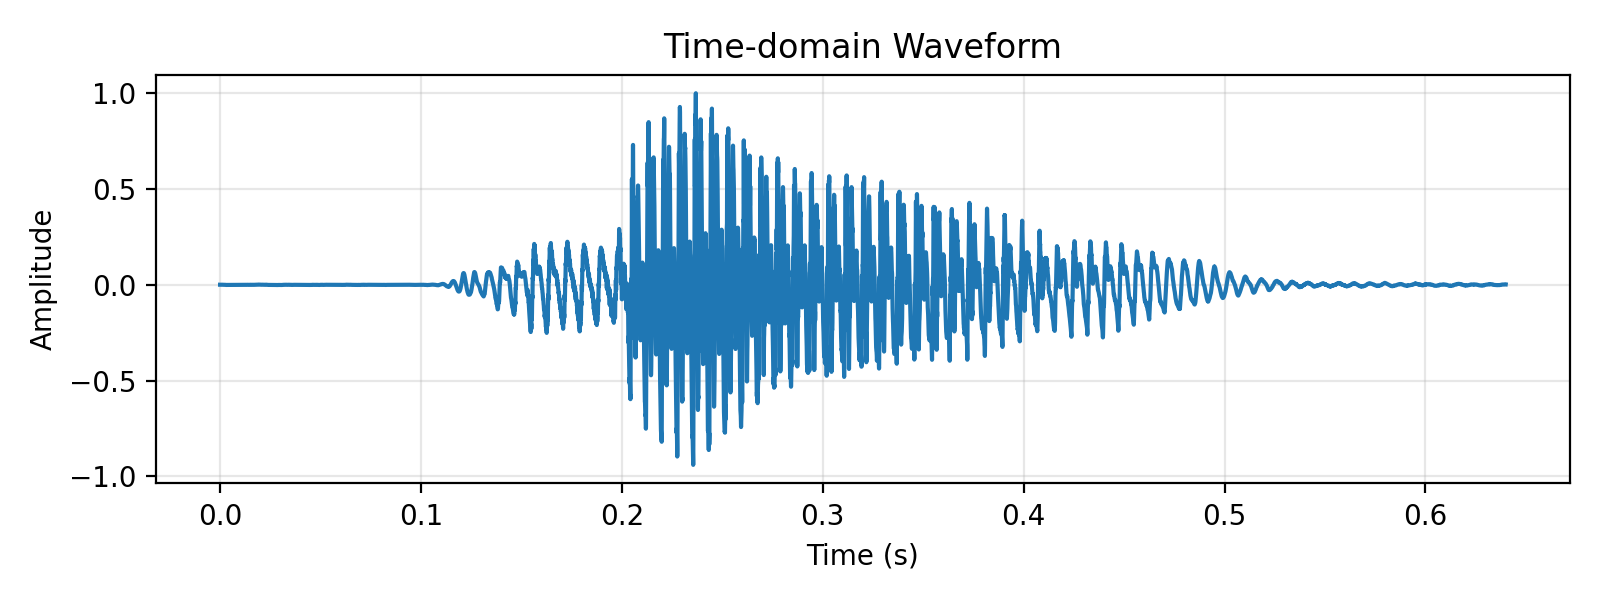
\includegraphics[width=0.80\textwidth]{waveform.png}\\[-6pt]
    {\footnotesize (a) 时域波形}

    \vspace{4pt}
    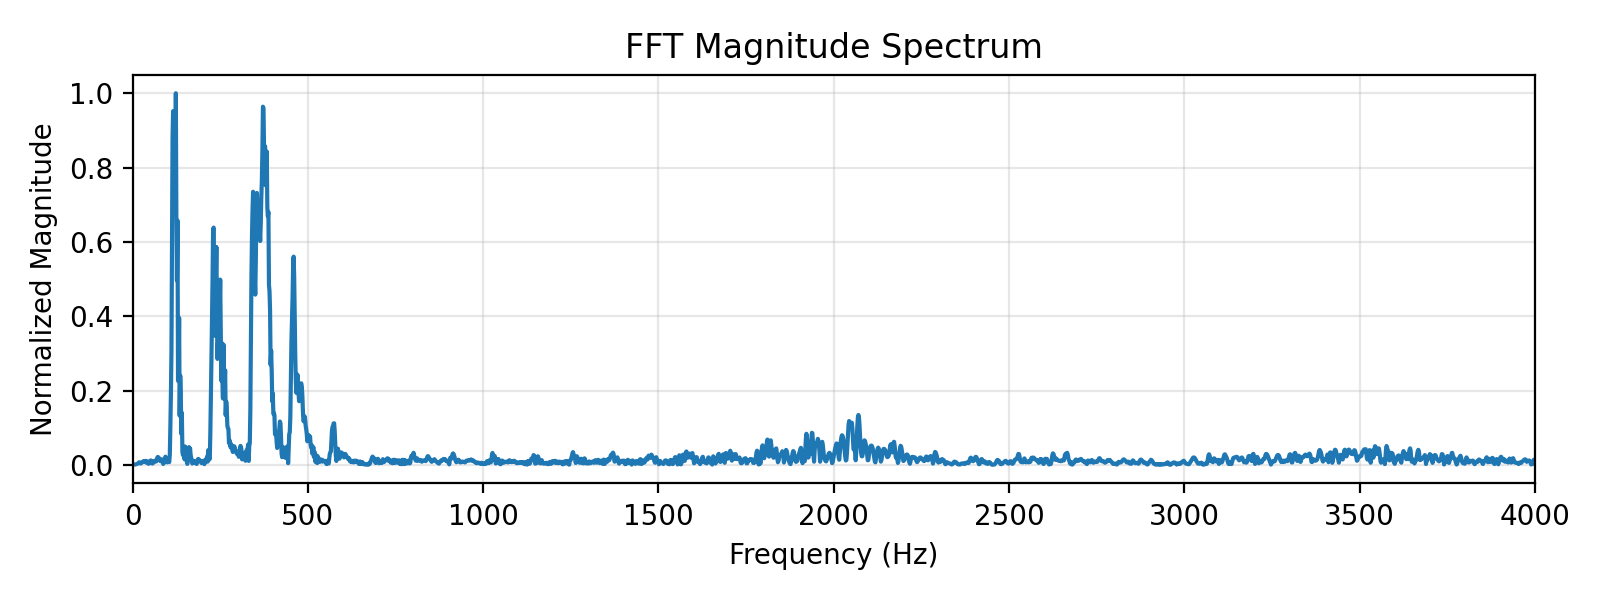
\includegraphics[width=0.80\textwidth]{fft_spectrum.png}\\[-6pt]
    {\footnotesize (b) FFT 幅度谱（0--4000 Hz）}

    \column{0.48\textwidth}
    \centering
    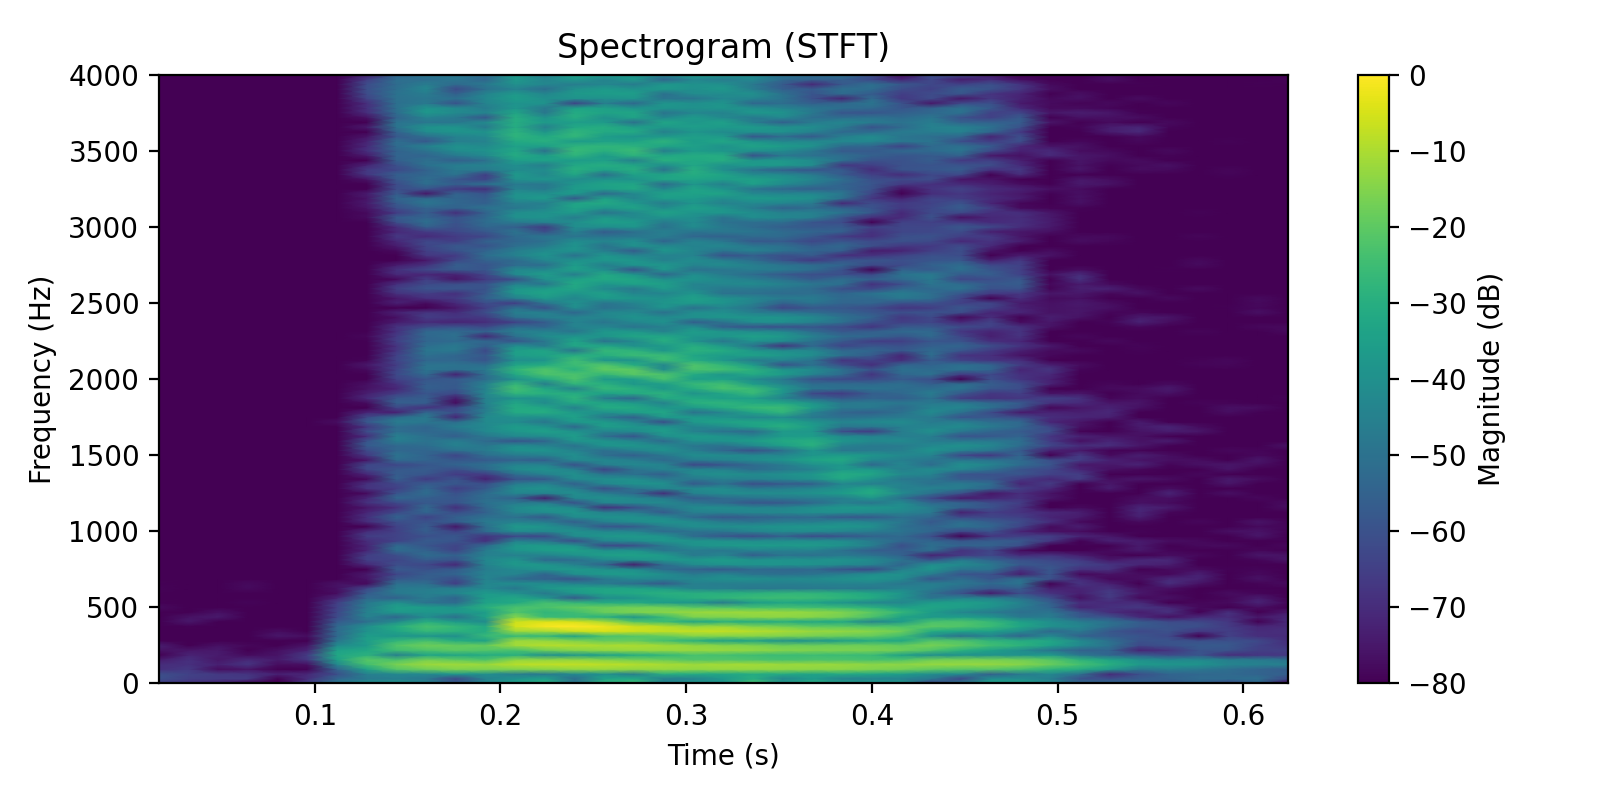
\includegraphics[width=0.80\textwidth]{spectrogram.png}\\[-6pt]
    {\footnotesize (c) STFT 语谱图}

    \medskip
    \raggedright\small
    语音是非平稳信号，单一 FFT 丢失频率随时间变化的信息。STFT 通过分帧加窗实现时频联合分析：
    \[
    \operatorname{STFT}\{x[n]\}(m,\omega) = \sum_{n=-\infty}^{\infty} x[n] w[n-mR] e^{-j\omega n}
    \]
    {\footnotesize 25 ms Hamming 窗，10 ms 帧移}
  \end{columns}
\end{frame}

\begin{frame}{MFCC 特征提取流程}
  \small
  \begin{columns}[T]
    \column{0.50\textwidth}
    \textbf{梅尔频率倒谱系数（MFCC）}
    \begin{enumerate}
      \setlength{\itemsep}{1pt}
      \item \textbf{预加重}：$y[n] = x[n] - 0.97 x[n-1]$（FIR 高通）
      \item \textbf{分帧加窗}：25 ms Hamming 窗，10 ms 帧移
      \item \textbf{FFT $\to$ 功率谱 $\to$ Mel 滤波}：26 个三角滤波器（低频密、高频疏）
      \item \textbf{取对数 + DCT}：压缩动态范围，去相关，取前 13 维
      \item \textbf{动态特征}：$\Delta$ 和 $\Delta^2$（一阶/二阶差分）$\to$ 39 维
    \end{enumerate}

    \column{0.46\textwidth}
    \centering
    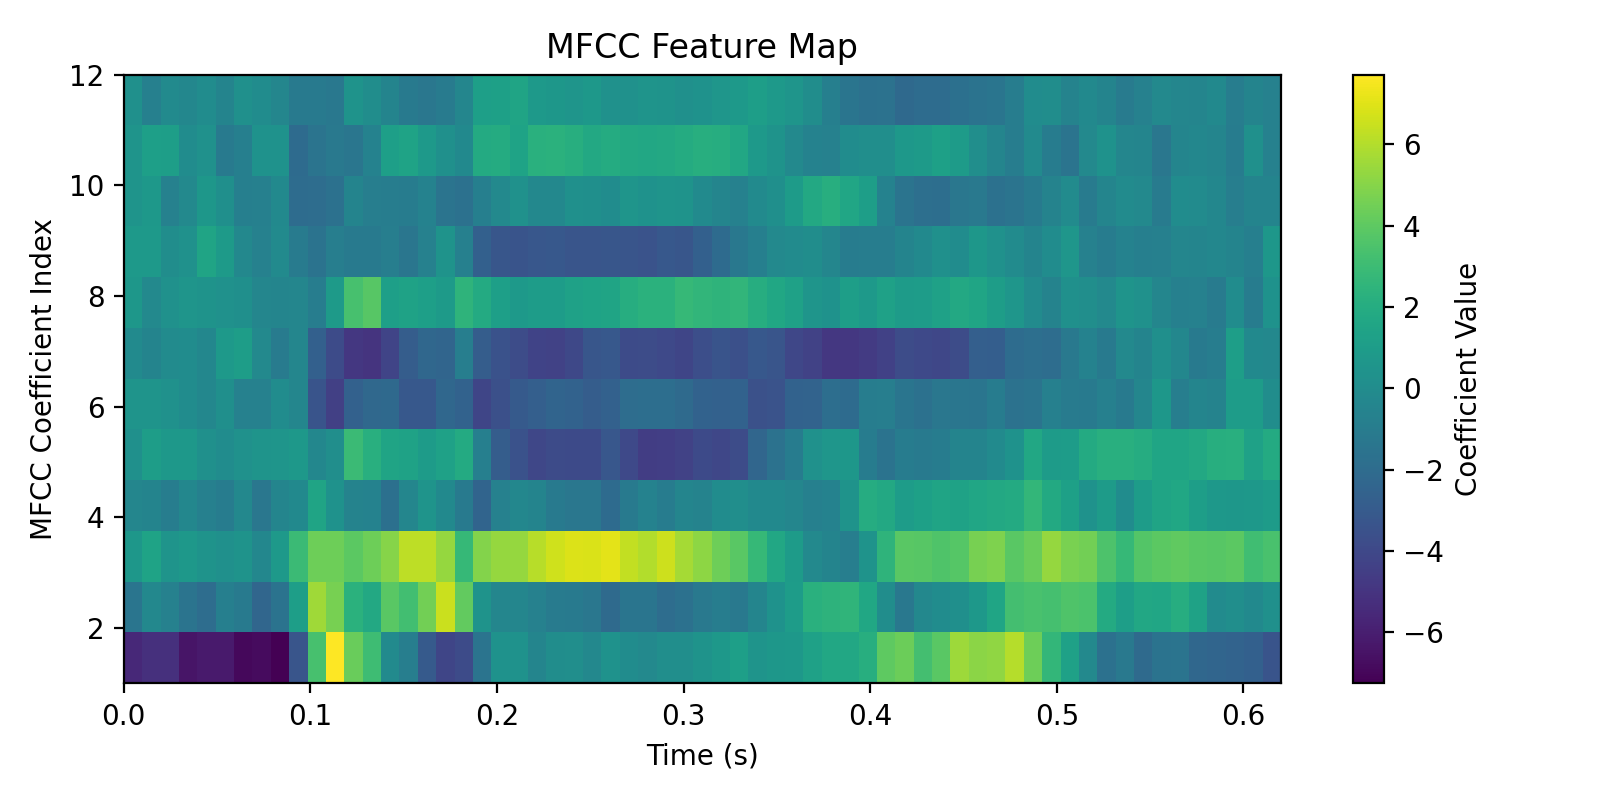
\includegraphics[width=0.80\textwidth]{mfcc.png}\\[-4pt]
    {\footnotesize 13 维 MFCC（传统方法）}

    \vspace{8pt}
    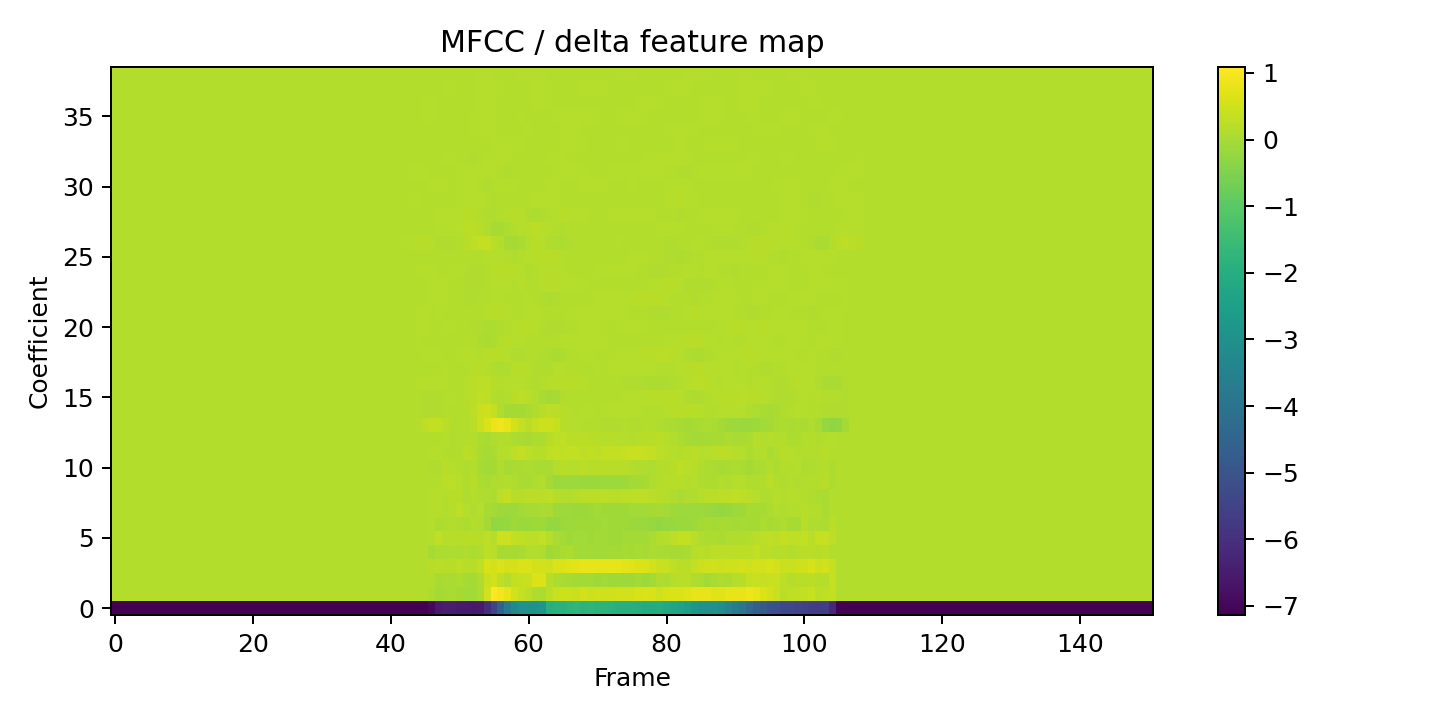
\includegraphics[width=0.80\textwidth]{mfcc_features.png}\\[-4pt]
    {\footnotesize 39 维 MFCC + $\Delta$ + $\Delta^2$（深度方法）}
  \end{columns}
\end{frame}

% !TeX encoding = UTF-8
% !TeX root = ../main.tex

\section{整体算法流程}

\begin{frame}{整体算法流程与信号处理关联}
  \centering
  \small
  \begin{tikzpicture}[
    node distance=0.55cm and 0.5cm,
    box/.style={draw, rounded corners=2pt, minimum width=0.85cm, minimum height=0.55cm,
                align=center, font=\footnotesize},
    pre/.style={box, fill=blue!12},
    feat/.style={box, fill=green!12},
    cls/.style={box, fill=orange!15},
    output/.style={box, fill=red!12},
    arr/.style={->, >=stealth, thick},
  ]

  % --- Row 1: Preprocessing ---
  \node[pre] (raw) {Raw\\MP3};
  \node[pre, right=of raw] (ed) {端点\\检测};
  \node[pre, right=of ed] (pe) {预加重\\$y[n]=x[n]-0.97x[n-1]$};
  \node[pre, right=of pe] (frame) {分帧加窗\\25ms Ham, 10ms hop};

  % --- Row 2: Feature Extraction ---
  \node[feat, right=of frame] (fft) {FFT\\$|\cdot|^2$};
  \node[feat, right=of fft] (mel) {Mel 滤波\\26 个三角};
  \node[feat, right=of mel] (logdct) {Log + DCT\\13 维};
  \node[feat, right=of logdct] (mfcc) {MFCC\\+ $\Delta$/$\Delta^2$\\39 维};

  % --- Row 3: Classification ---
  \node[cls, below=1.0cm of mfcc] (clf) {KNN / GMM / CNN};
  \node[output, right=of clf] (pred) {预测\\0--9};

  % --- Arrows ---
  \draw[arr] (raw) -- (ed);
  \draw[arr] (ed) -- (pe);
  \draw[arr] (pe) -- (frame);
  \draw[arr] (frame) -- (fft);
  \draw[arr] (fft) -- (mel);
  \draw[arr] (mel) -- (logdct);
  \draw[arr] (logdct) -- (mfcc);
  \draw[arr] (mfcc.south) -- ++(0,-0.35) -| (clf.north);
  \draw[arr] (clf) -- (pred);

  % --- Labels ---
  \node[font=\footnotesize\bfseries, above=0.15cm of raw.north, anchor=south] {预处理};
  \node[font=\footnotesize\bfseries, above=0.15cm of fft.north, anchor=south] {特征提取};
  \node[font=\footnotesize\bfseries, below=0.15cm of clf.south, anchor=north] {分类器};

  \end{tikzpicture}

  \medskip
  \begin{columns}[T]
    \column{0.48\textwidth}
    \begin{block}{两条技术路线}
      \footnotesize
      \begin{itemize}
        \item \textbf{传统方法}：手工特征 + KNN（统计）/ GMM（序列）
        \item \textbf{深度方法}：MFCC 特征图 + 卷积神经网络（TinyKeywordCNN）
      \end{itemize}
    \end{block}

    \column{0.48\textwidth}
    \begin{block}{信号与系统核心关联}
      \footnotesize
      \begin{itemize}
        \item FFT：时域到频域的桥梁
        \item STFT：非平稳信号的时频联合分析
        \item Mel 滤波器组：模拟人耳非线性频率感知
        \item DCT：频域去相关与能量压缩
        \item 预加重/分帧加窗：FIR 滤波与短时平稳假设
      \end{itemize}
    \end{block}
  \end{columns}
\end{frame}

% !TeX encoding = UTF-8
% !TeX root = ../main.tex

\section{识别方法}

\begin{frame}{传统方法一：MFCC 统计特征 + KNN}
  \begin{columns}[T]
    \column{0.55\textwidth}
    \textbf{特征构造}
    \begin{itemize}
      \item 每段语音提取 13 维 MFCC，逐帧取均值与标准差
      \item 拼接为固定 26 维特征向量：
            \[
            \mathbf{f} = [\boldsymbol{\mu}_{\text{MFCC}}\ \ \boldsymbol{\sigma}_{\text{MFCC}}]
            \]
      \item 优点：简单、可解释、适合小样本
      \item 缺点：丢失时间顺序信息
    \end{itemize}

    \medskip
    \textbf{分类器}
    \begin{itemize}
      \item StandardScaler 标准化
      \item 1-NN（$k=1$，欧氏距离）分类器
      \item 训练：50 样本，验证：20 样本
    \end{itemize}

    \column{0.40\textwidth}
    \centering
    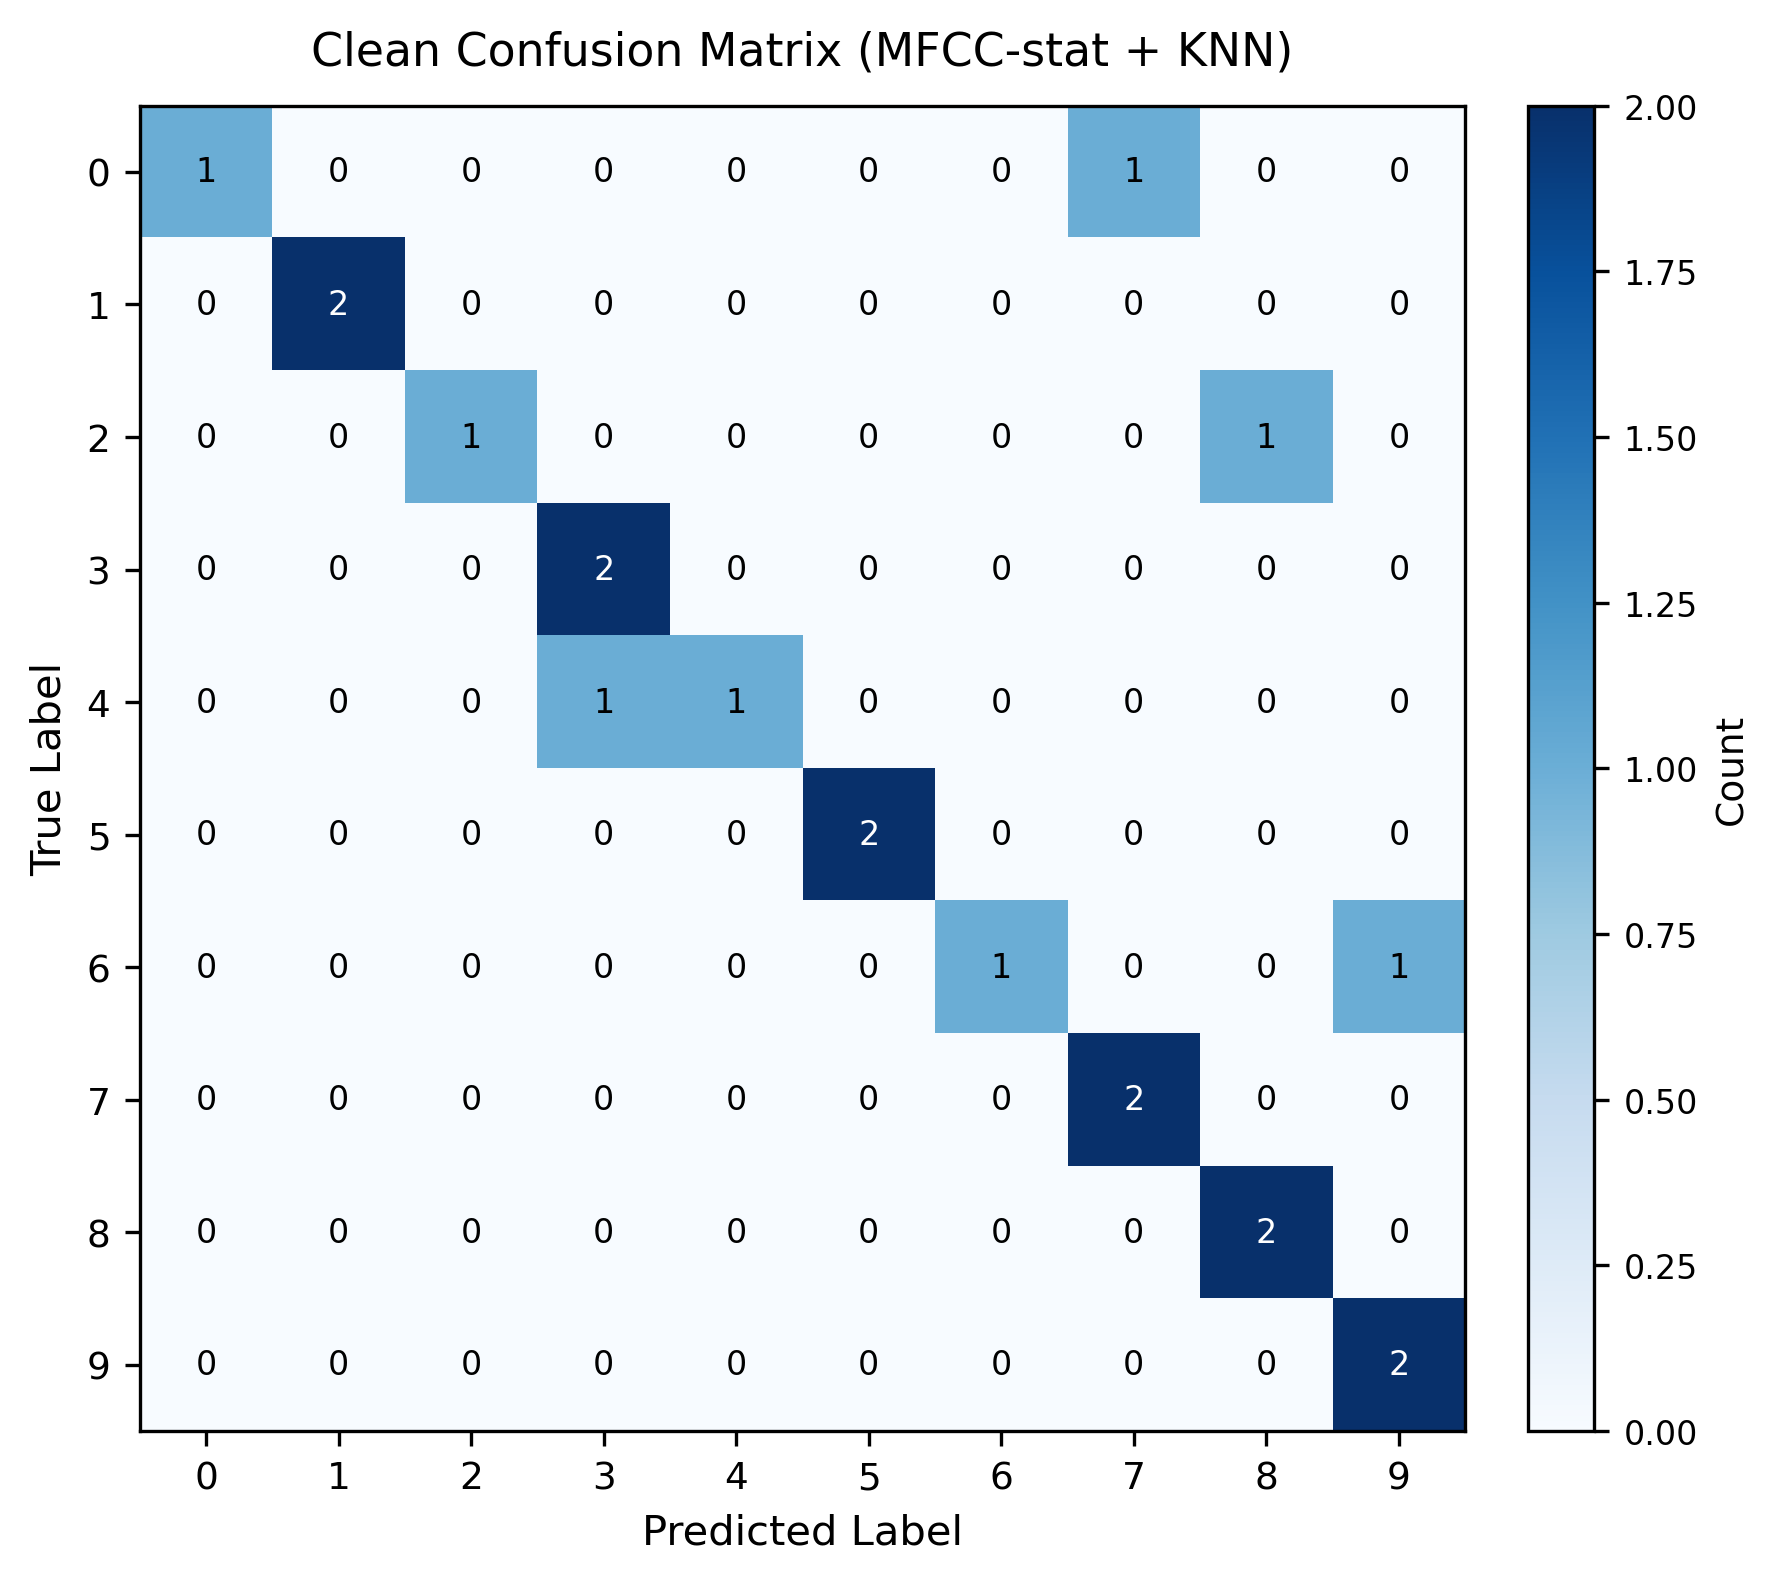
\includegraphics[width=\textwidth]{../results/traditional/baseline_knn/figures/clean_confusion_matrix.png}\\[-4pt]
    {\footnotesize 纯净语音混淆矩阵}

    \medskip
    \begin{itemize}
      \item 纯净准确率：\alert{80.0\%}（16/20）
      \item 主要混淆：$0\to7$, $2\to8$, $4\to3$, $6\to9$
    \end{itemize}
  \end{columns}
\end{frame}

\begin{frame}{传统方法二：MFCC + $\Delta$ + $\Delta^2$ + GMM}
  \begin{columns}[T]
    \column{0.52\textwidth}
    \textbf{特征改进}
    \begin{itemize}
      \item 13 维 MFCC + $\Delta$ + $\Delta^2$ = 39 维序列特征
      \item 动态特征捕获时间演变信息
      \item CMVN（倒谱均值方差归一化）：提升对信道变化的鲁棒性
    \end{itemize}

    \medskip
    \textbf{高斯混合模型（GMM）}
    \begin{itemize}
      \item 每类数字训练一个 4 分量对角协方差 GMM
      \item 判决：对数似然最大
            \[
            \hat{y} = \arg\max_{c\in\{0,\dots,9\}} \sum_{t=1}^{T} \log p(\mathbf{x}_t \mid \lambda_c)
            \]
      \item GMM 天然适合序列特征：无需压缩为固定维度
    \end{itemize}

    \column{0.43\textwidth}
    \centering
    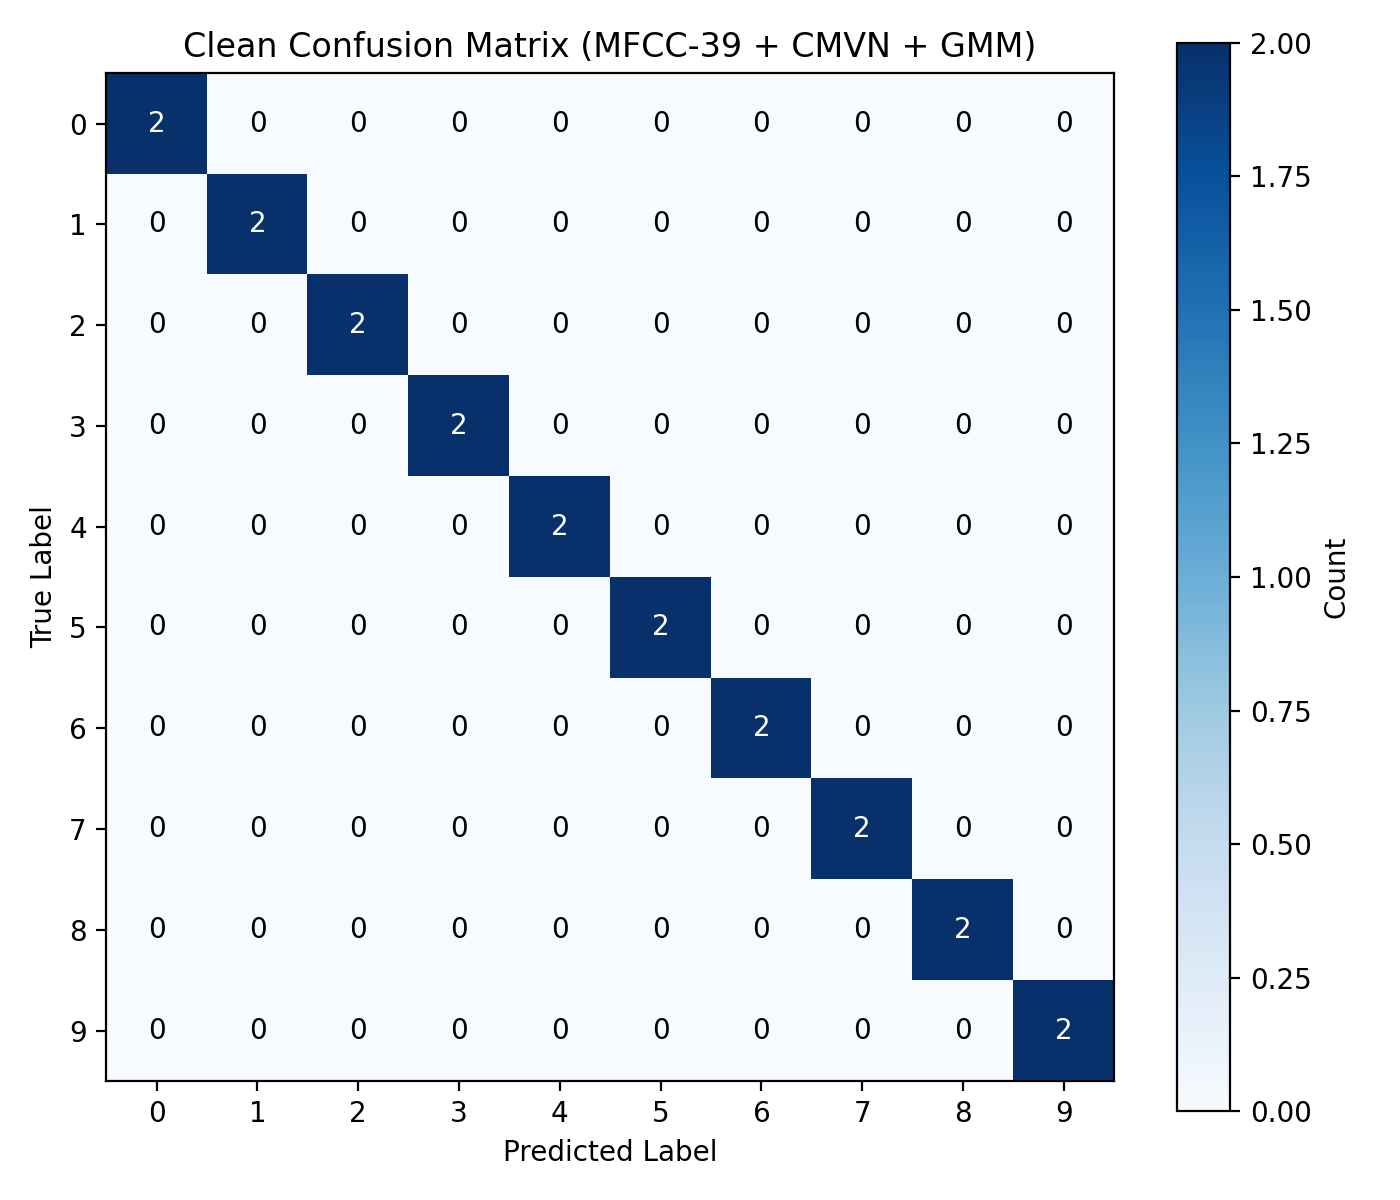
\includegraphics[width=\textwidth]{../results/traditional/advanced_gmm/figures/clean_confusion_matrix.png}\\[-4pt]
    {\footnotesize 纯净语音混淆矩阵}

    \medskip
    \begin{itemize}
      \item 纯净准确率：\alert{100.0\%}（20/20）
      \item 全部正确分类，无混淆
    \end{itemize}
  \end{columns}
\end{frame}

\begin{frame}{深度学习方法：TinyKeywordCNN}
  \begin{columns}[T]
    \column{0.52\textwidth}
    \textbf{特征与模型}
    \begin{itemize}
      \item 输入：MFCC + $\Delta$ + $\Delta^2$，$39 \times T$ 特征图
      \item 4 个卷积块（Conv2d $\to$ BatchNorm $\to$ ReLU）：
            \[
            1 \to 16 \to 32 \to 64 \to 128 \text{ 通道}
            \]
      \item MaxPooling 逐步降采样
      \item AdaptiveAvgPool(2,2) + Dropout(0.3) + Linear $\to$ 10
      \item 总参数量：\alert{102,522}
    \end{itemize}

    \medskip
    \textbf{训练策略}
    \begin{itemize}
      \item 优化器：AdamW（lr=0.001, weight\_decay=1e-4）
      \item 数据增强：随机增益 $\pm 3$ dB、时间平移 $\pm 120$ ms、
            随机加噪（$p=0.3$, SNR 0--20 dB）
      \item 早停（patience=20, max 120 epochs），
            最优轮次：epoch 37
    \end{itemize}

    \column{0.43\textwidth}
    \centering
    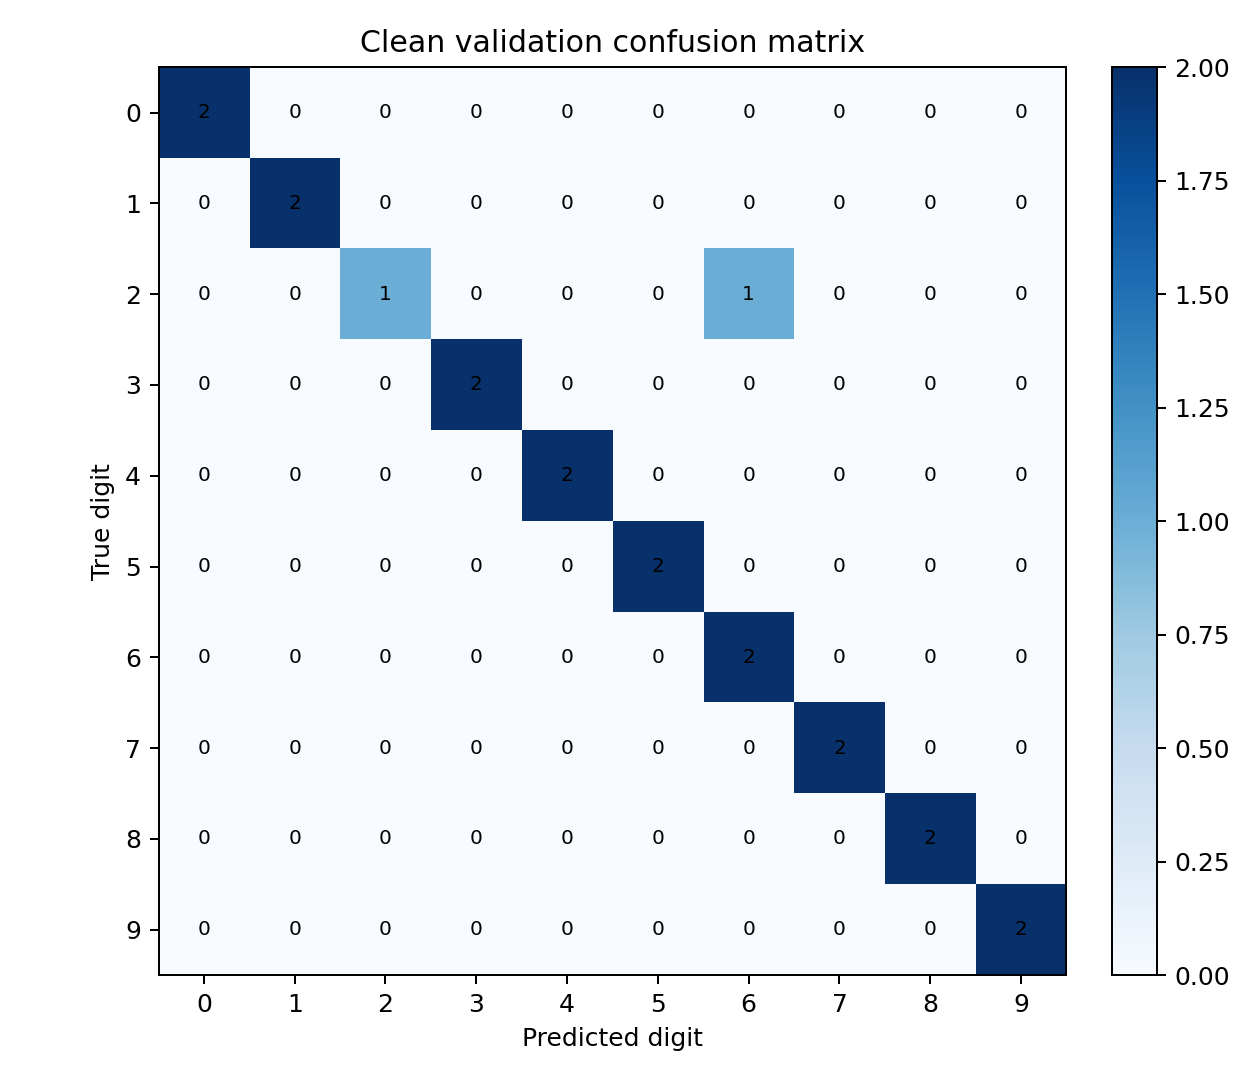
\includegraphics[width=\textwidth]{../outputs/deep_learning/clean_confusion_matrix.png}\\[-4pt]
    {\footnotesize 纯净语音混淆矩阵}

    \medskip
    \begin{itemize}
      \item 纯净准确率：\alert{95.0\%}（19/20）
      \item 1 个错误：数字 2 误判为 6
    \end{itemize}
  \end{columns}
\end{frame}

% !TeX encoding = UTF-8
% !TeX root = ../main.tex

\section{结果分析与总结}

\begin{frame}{纯净语音识别结果对比}
  \small
  \begin{columns}[T]
    \column{0.56\textwidth}
    \centering
    \textbf{纯净语音识别结果}
    \vspace{4pt}

    \begin{tabular}{lcc}
      \toprule
      \textbf{方法} & \textbf{维度} & \textbf{准确率} \\
      \midrule
      MFCC-stat + KNN   & 26 维 & 80.0\% \\
      MFCC+$\Delta$/$\Delta^2$+GMM & 39 维 & \alert{100.0\%} \\
      TinyKeywordCNN (102k) & 39 维 & 95.0\% \\
      \bottomrule
    \end{tabular}

    \vspace{8pt}
    \raggedright
    \begin{itemize}
      \setlength{\itemsep}{2pt}
      \item GMM：20 条验证样本全部识别正确
      \item CNN：1 个误判（$2\to6$）
      \item KNN：4 个混淆，说明统计特征丢失了部分时序信息
    \end{itemize}

    \column{0.38\textwidth}
    \textbf{对比结论}
    \begin{itemize}
      \setlength{\itemsep}{4pt}
      \item 动态特征能补充语音变化趋势
      \item GMM 保留变长序列信息，适合小样本任务
      \item CNN 具有端到端建模能力，但本实验验证集较小
    \end{itemize}
  \end{columns}
\end{frame}

\begin{frame}{噪声鲁棒性：KNN 基线}
  \small
  \begin{columns}[T]
    \column{0.62\textwidth}
    \centering
    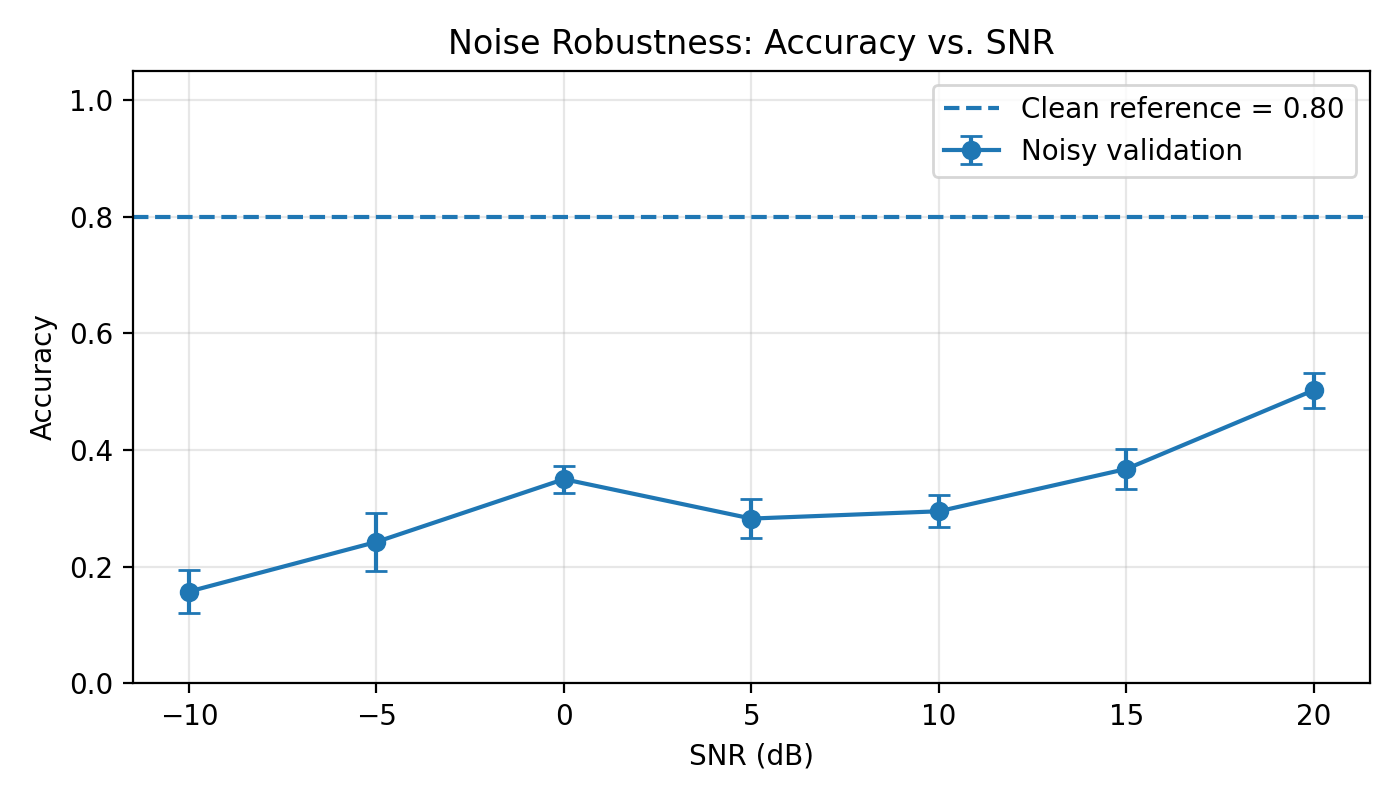
\includegraphics[width=0.95\textwidth]{../results/traditional/noise_robustness_v2/accuracy_snr_curve_mean_std.png}

    \column{0.34\textwidth}
    \textbf{MFCC-stat + KNN}
    \begin{itemize}
      \setlength{\itemsep}{4pt}
      \item 每个 SNR 重复 20 次，曲线展示均值与波动范围
      \item 低 SNR 下准确率明显下降
      \item 最高 SNR 下仍未达到 90\%，说明均值/标准差统计特征鲁棒性有限
    \end{itemize}
  \end{columns}
\end{frame}

\begin{frame}{噪声鲁棒性：GMM 序列模型}
  \small
  \begin{columns}[T]
    \column{0.62\textwidth}
    \centering
    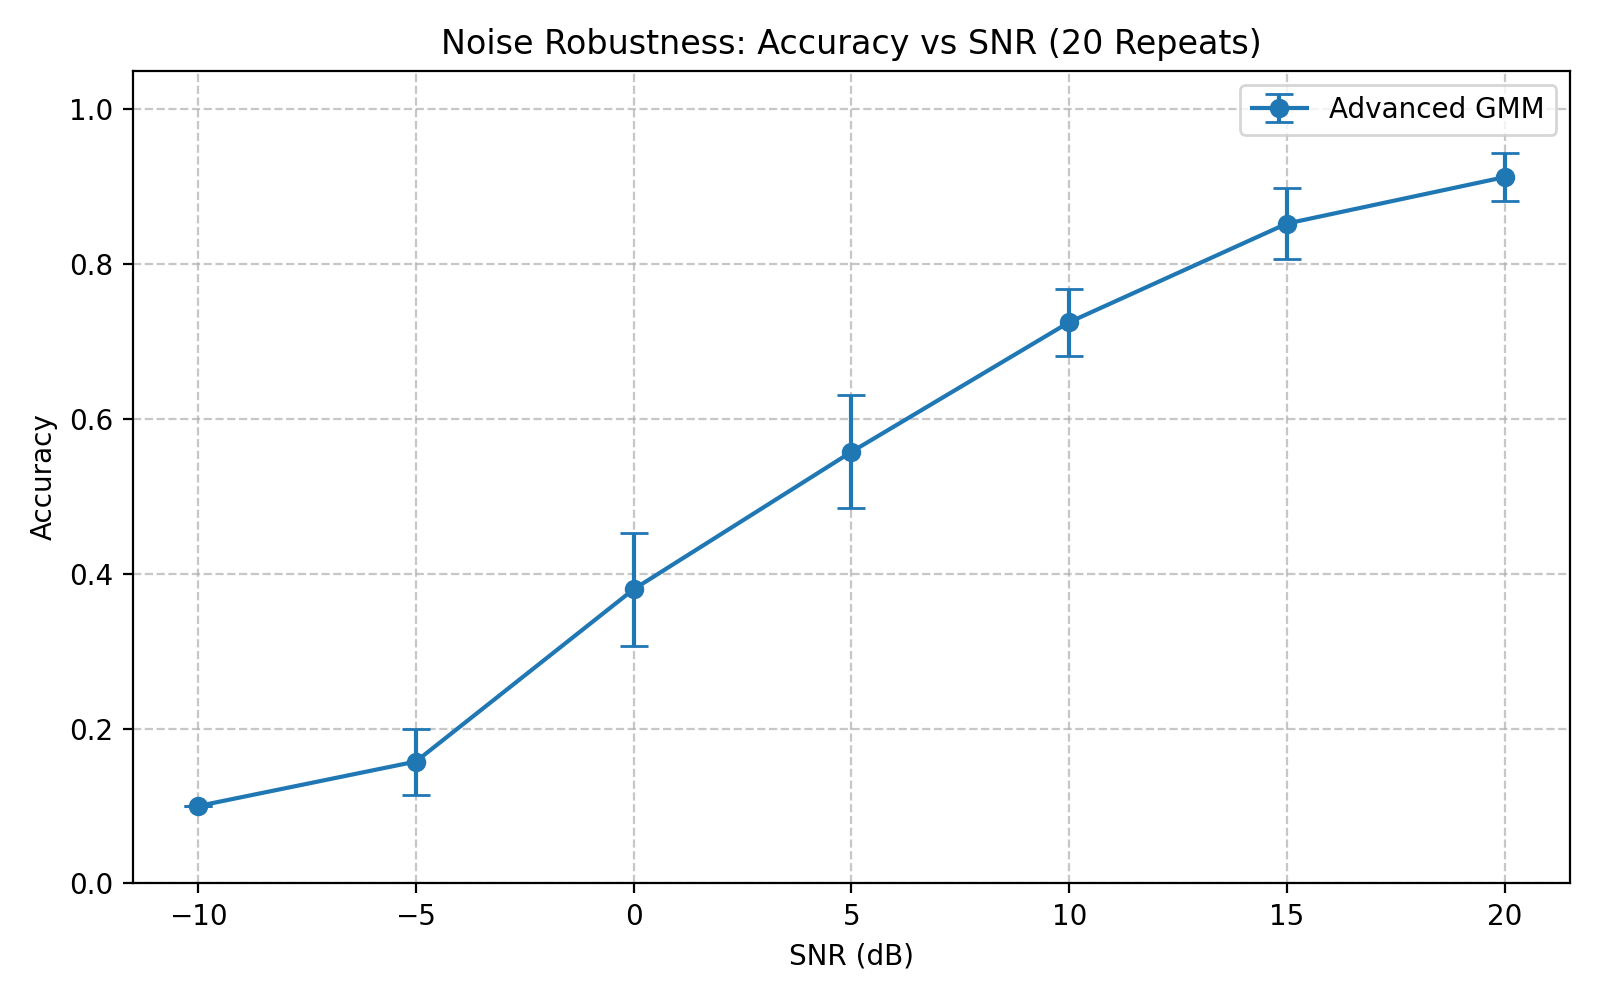
\includegraphics[width=0.95\textwidth]{../results/traditional/advanced_gmm/figures/accuracy_snr_curve.png}

    \column{0.34\textwidth}
    \textbf{MFCC + $\Delta$ + $\Delta^2$ + GMM}
    \begin{itemize}
      \setlength{\itemsep}{4pt}
      \item 引入动态特征与 CMVN 归一化
      \item 中高 SNR 下性能提升明显
      \item 在 20 dB 时达到 90\% 以上准确率（91.25\%）
    \end{itemize}
  \end{columns}
\end{frame}

\begin{frame}{噪声鲁棒性：TinyKeywordCNN}
  \small
  \begin{columns}[T]
    \column{0.62\textwidth}
    \centering
    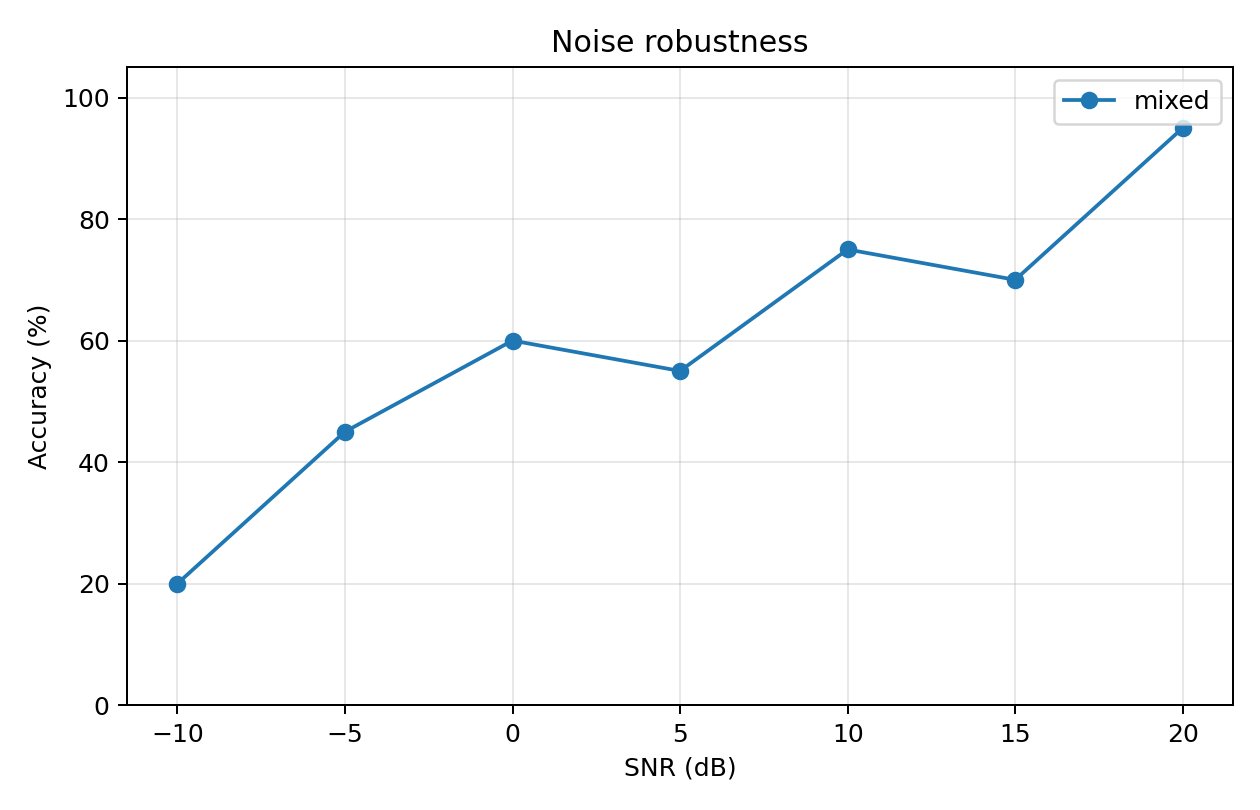
\includegraphics[width=0.95\textwidth]{../outputs/deep_learning/accuracy_snr_curve.png}

    \column{0.34\textwidth}
    \textbf{MFCC 特征图 + CNN}
    \begin{itemize}
      \setlength{\itemsep}{4pt}
      \item 训练中加入增益、平移和随机噪声增强
      \item 低 SNR 下相对更稳
      \item CNN 为单次测试，统计意义与 KNN/GMM 的重复均值不完全等价
    \end{itemize}
  \end{columns}
\end{frame}

\begin{frame}{总结与局限性}
  \footnotesize
  \begin{columns}[T,totalwidth=\textwidth]
    \column{0.51\textwidth}
    \textbf{\large 核心结论}
    \vspace{2pt}
    \begin{enumerate}
      \setlength{\itemsep}{3pt}
      \item MFCC 能有效刻画孤立数字语音的谱包络差异，是本任务的关键声学特征。
      \item KNN 基线简单可解释，但均值/标准差统计会丢失时序信息，鲁棒性较弱。
      \item GMM 保留变长序列特征，在纯净语音和中高 SNR 下表现最稳定；在 20 dB 时准确率达到 90% 以上。
      \item TinyKeywordCNN 受益于数据增强，在低 SNR 下表现相对平稳。
    \end{enumerate}

    \vspace{5pt}
    \textbf{\large 局限性}
    \vspace{2pt}
    \begin{itemize}
      \setlength{\itemsep}{2pt}
      \item 验证集仅 20 条，结果存在一定偶然性，统计意义有限
      \item 仅测试统一混合噪声，未拆分单类噪声影响
      \item 未进行说话人交叉验证
    \end{itemize}
  \end{columns}

  \textbf{\large 团队分工}
    \vspace{2pt}
    \begin{itemize}
      \setlength{\itemsep}{2pt}
      \item 于沛龙：传统方法基线、噪声鲁棒性测试、PPT 整理
      \item 景序：GMM 序列模型、传统方法优化与结果分析
      \item 封宇凡：深度学习模型设计、训练与评估
      \item 孟德轩：数据处理、实验对照、报告与展示材料整理
    \end{itemize}
\end{frame}

\makebottom

\end{document}
